\documentclass[serif, 12pt]{beamer}

\usepackage{graphicx} % Allows including images
\usepackage{booktabs} % Allows the use of \toprule, \midrule and \bottomrule in tables

\usepackage{color}

%\usepackage{algorithm2e}
\usepackage{hyperref}
\usepackage{algorithm,algorithmic}
\usepackage{changepage}
\usepackage{pgfplots}
\usepackage{pgfplotstable}
\usepgfplotslibrary{statistics}

\newcommand*\mat[1]{ \begin{pmatrix} #1 \end{pmatrix}}
\newcommand*\arr[1]{ \begin{bmatrix} #1 \end{bmatrix}}
\newcommand*\V[1]{ \boldsymbol{#1}}

\newcommand*\D{\textcolor{violet}{D}}
\newcommand*\T{\textcolor{blue}{T}}

\setbeamertemplate{navigation symbols}{}%remove navigation symbols

\setbeamerfont{page number in head/foot}{size=\small}
\setbeamertemplate{footline}[frame number]

\title{Approximated PCA}
\subtitle{Iteration 3}

\author{Rodrigo Arias} % Your name
\date{\today} % Date, can be changed to a custom date

\begin{document}

\begin{frame}
	\titlepage
\end{frame}

%------------------------------------------------

\begin{frame}

\frametitle{Proposed hypothesis}

Let $\epsilon_b$ be the error in the result with width $b$, then the following 
hypothesis can be proposed:
\begin{itemize}
\item The mean of $\log_2(\epsilon_b) \approx -b$.
\item The standard deviation $\approx 2$.
\end{itemize}

\end{frame}

%------------------------------------------------

%\begin{frame}
%\frametitle{Mean}
%Let $X_b = \log_2(\epsilon_b)$ be a random variable with unknown mean $\mu_X$ 
%and variance $\sigma^2$.  Then, after $k$ runs, the observed mean $\overline x$ 
%follows (CLT):
%%
%$$ \overline X = \frac{X_b^{(1)} + \dots + X_b^{(k)}}{k} \sim 
%N(\mu_X,\sigma/\sqrt k)$$
%%
%Or:
%%
%$$ Z = \frac{\overline X - \mu_X}{\sigma/\sqrt{k}} \sim N(0, 1)$$
%\end{frame}

%------------------------------------------------

\begin{frame}
\frametitle{Exploratory data analysis}
The technique was proposed by John Tukey to staticians, to explore new data.  
The method works in three main steps:
%The proposed approach consists in analyzing the data by visual inspection, 
%following by the formulation of hypothesis and testing them.

\begin{enumerate}
\item Inspect visually
\item Propose hypothesis
\item Test the proposed hypothesis
\end{enumerate}
\end{frame}
%------------------------------------------------

\begin{frame}
\frametitle{Definition of $X_b$}
\begin{itemize}
\item Considering the experiments performed with the bit-width $b$.

\item With $\epsilon_b$ being the measure of the rounding error, let $X_b = 
\log_2(\epsilon_b)$ be a random variable.

\item Then, after $k$ runs, we obtain the sample means $\overline X_b$ for all 
values tested of $b$.
\end{itemize}
%%
%$$ \overline X = \frac{X_b^{(1)} + \dots + X_b^{(k)}}{k} \sim 
%N(\mu_X,\sigma/\sqrt k)$$
%%
%Or:
%%
%$$ Z = \frac{\overline X - \mu_X}{\sigma/\sqrt{k}} \sim N(0, 1)$$
\end{frame}

%------------------------------------------------

%\begin{frame}
%\frametitle{Mean}
%For any $\alpha$, $0 < \alpha < 1$, let $z_\alpha$ be such that $P[Z>z_\alpha] = 
%\alpha$
%
%With probability $1-\alpha$, the mean $\mu$ will lie in the region:
%%
%$$\overline X \pm z_{\alpha/2}S/\sqrt{n}$$
%\end{frame}

%------------------------------------------------

\begin{frame}

\frametitle{Plot of the sample mean error $\overline X_b$}

\begin{figure}[h]
	\begin{tikzpicture}
		\begin{axis}[
%			scale only axis,
			xlabel={$b$},
			ylabel={$\overline X_b$},
			height=0.8*\textheight,
			grid = both,
		]
			\addplot+ [
				mark=none,
%				only marks,
%				mark size = 0.5pt
			] table [
				x index = {0},
				y index = {1},
				col sep = space
			] {../data/exp1a.csv};
		\end{axis}
	\end{tikzpicture}
	%\includegraphics[width=\textwidth]{bighh}
	\caption{Plot of $\overline X_b$ as the number of bits $b$ increases.}
	\label{fig:errhh}
\end{figure}

\end{frame}

%------------------------------------------------

\begin{frame}

\frametitle{Difference with $b$}

It seems that $\overline X_b$ is almost $-b$. To see if there is any difference, 
we can plot $b + \overline X_b$, and check if the mean of the result is 0.

\end{frame}

%------------------------------------------------

\begin{frame}

\frametitle{Plot of the difference}

\begin{figure}[h]
	\begin{tikzpicture}
		\begin{axis}[
%			scale only axis,
			xlabel={$b$},
			ylabel={$b + \overline X_b$},
			height=0.8*\textheight,
			grid = both,
		]
			\addplot+ [
				mark=none,
%				only marks,
%				mark size = 0.5pt
			] table [
				x index = {0},
				y index = {1},
				col sep = space
			] {../data/exp1f.csv};
		\end{axis}
	\end{tikzpicture}
	%\includegraphics[width=\textwidth]{bighh}
	\caption{Plot of $b + \overline X_b$ as the number of bits $b$ increases.}
	\label{fig:errhh}
\end{figure}

\end{frame}

%------------------------------------------------

\begin{frame}

\frametitle{Deviation on lower bits}

There can be seen that when $b < 5$, the error deviates from the mean. Lets 
ignore those values as outliers. And check again the plot.

\end{frame}

%------------------------------------------------

\begin{frame}

\frametitle{Plot of the difference}

\begin{figure}[h]
	\begin{tikzpicture}
		\begin{axis}[
%			scale only axis,
			xlabel={$b$},
			ylabel={$b + \overline X_b$},
			height=0.8*\textheight,
			grid = both,
		]
			\addplot+ [
				mark=none,
%				only marks,
%				mark size = 0.5pt
			] table [
				x index = {0},
				y index = {1},
				col sep = space
			] {../data/exp1f2.csv};
		\end{axis}
	\end{tikzpicture}
	%\includegraphics[width=\textwidth]{bighh}
	\caption{Plot of $b + \overline X_b$ as the number of bits $b$ increases.}
	\label{fig:errhh}
\end{figure}

\end{frame}

%------------------------------------------------

\begin{frame}

\frametitle{Histogram of the difference}

\begin{figure}[h]
	\begin{tikzpicture}
		\begin{axis}[
%			scale only axis,
			ybar,
			height=0.8*\textheight,
			grid = both,
%			xmin=0,xmax=100
		]
			\addplot+ [
				hist={bins=15},
				mark=none,
%				only marks,
%				mark size = 0.5pt
			] table [
				x index = {0},
				y index = {1},
				col sep = space
			] {../data/exp1f2.csv};

		\end{axis}
	\end{tikzpicture}
	%\includegraphics[width=\textwidth]{bighh}
	\caption{Histogram of the difference $\overline b+X_b$}
	\label{fig:errhh}
\end{figure}

\end{frame}

%------------------------------------------------

\begin{frame}

\frametitle{Distribution of the error}

Now the difference seems to be a random variable, with a fixed mean $\mu$ 
independent of $b$.
%
Let $Y = b + \overline X_b$. Then,
%
$$ \overline X_b = -b + Y $$
%
By the central limit theorem, with probability $1-\alpha$, the mean $\mu$ will 
lie in the region:
%
$$\overline Y \pm z_{\alpha/2}S/\sqrt{n}$$
%
%The mean $\mu$ is in the region $(2.68974, 2.68409)$ with 99.9\% of confidence.
The mean $\mu$ is in $2.68691\pm0.00190$ with 95\% of confidence.
%Let $\mu$ be the mean of $Y$, then the difference of the sample mean $\overline 
%Y$ with $\mu$ is:
%
%$$ \overline Y \sim N(\mu,\sigma/\sqrt k)$$
%%
%Or:
%%
%$$ Z = \frac{\overline X - \mu}{\sigma/\sqrt{k}} \sim N(0, 1)$$
%%
%For any $\alpha$, $0 < \alpha < 1$, let $z_\alpha$ be such that $P[Z>z_\alpha] = 
%\alpha$
%
%With probability $1-\alpha$, the mean $\mu$ will lie in the region:
%%
%$$\overline X \pm z_{\alpha/2}S/\sqrt{n}$$



\end{frame}

%------------------------------------------------

\begin{frame}

\frametitle{Plot of the difference}

\begin{figure}[h]
	\begin{tikzpicture}
		\begin{axis}[
%			scale only axis,
			xlabel={$b$},
			ylabel={$b + \overline X_b$},
			height=0.8*\textheight,
			grid = both,
			xmin=0,xmax=100
		]
			\addplot+ [
				mark=none,
%				only marks,
%				mark size = 0.5pt
			] table [
				x index = {0},
				y index = {1},
				col sep = space
			] {../data/exp1f2.csv};

			\addplot+ [mark=none, red]
				coordinates {(0, 2.68691+0.00190) (100, 2.68691+0.00190)};
			\addplot+ [mark=none, red]
				coordinates {(0, 2.68691-0.00190) (100, 2.68691-0.00190)};
		\end{axis}
	\end{tikzpicture}
	%\includegraphics[width=\textwidth]{bighh}
	\caption{The mean $\mu$ is in the marked region with 95\% confidence.}
	\label{fig:errhh}
\end{figure}

\end{frame}

%------------------------------------------------

\begin{frame}

\frametitle{Test of independence}

\begin{itemize}

\item To determine if the error is dependent of the bit-width $b$, a correlation 
test can be performed.

\item The null hypothesis is that $Y$ is dependent of $b$. The correlation 
coefficient is $-0.222$ and the p-value $0.02969$.

\item So we can reject the null hypothesis, and assume that they are 
independent.
\end{itemize}

\end{frame}

%------------------------------------------------

\begin{frame}

\frametitle{Conclusions about the mean $\overline X_b$}

\begin{itemize}

\item $\overline X_b$ is proportional to $b$. Can be described as $\overline X_b 
= -b + Y$.

\item The random variable $Y$ is independent of $b$.

\item There is a strange behavior when $b<5$, where $\overline X_b$ don't follow 
the expected value. The cause of this behavior is yet unknown.

\item More experiments are needed, to test if $X_b$ depends on the input size 
$N$.

\end{itemize}

\end{frame}

%------------------------------------------------

\begin{frame}

\frametitle{Observation of the standard deviation}

The sample standard deviation $S$ can be observed for each bit-width $b$.

\vspace{1em}

Let $S_b$ be the sample s.d. of $X_b$ in the $k$ runs.

\vspace{1em}

Note that the real standard deviation $\sigma_b$ is unknown, but $S_b$ is an 
unbiased estimator of $\sigma_b$

\end{frame}

%------------------------------------------------

\begin{frame}

\frametitle{Plot of the standard deviation}

\begin{figure}[h]
	\begin{tikzpicture}
		\begin{axis}[
%			scale only axis,
			xlabel={$b$},
			ylabel={$S_b$},
			height=0.8*\textheight,
			grid = both,
			xmin=0,xmax=100
		]
			\addplot+ [
				mark=none,
%				only marks,
%				mark size = 0.5pt
			] table [
				x index = {0},
				y index = {1},
				col sep = space
			] {../data/exp2g.csv};

		\end{axis}
	\end{tikzpicture}
	%\includegraphics[width=\textwidth]{bighh}
	\caption{The sample standard deviation $S_b$ as the bit-width $b$ grows.}
	\label{fig:errhh}
\end{figure}

\end{frame}

%------------------------------------------------

\begin{frame}

\frametitle{Deviation on lower bits}

Again, there is a deviation from the mean on the lower bits, now when $b < 12$.  
Those values will be ignored as outliers.

Also, the mean of the standard deviation seems to be near $0.9$ not $2$.


\end{frame}

%------------------------------------------------

\begin{frame}

\frametitle{Plot of the standard deviation}

\begin{figure}[h]
	\begin{tikzpicture}
		\begin{axis}[
%			scale only axis,
			xlabel={$b$},
			ylabel={$S_b$},
			height=0.8*\textheight,
			grid = both,
			xmin=0,xmax=100
		]
			\addplot+ [
				mark=none,
%				only marks,
%				mark size = 0.5pt
			] table [
				x index = {0},
				y index = {1},
				col sep = space
			] {../data/exp1g2.csv};

		\end{axis}
	\end{tikzpicture}
	%\includegraphics[width=\textwidth]{bighh}
	\caption{The sample standard deviation $S_b$ as the bit-width $b$ grows.}
	\label{fig:errhh}
\end{figure}

\end{frame}

%------------------------------------------------

\begin{frame}

\frametitle{Histogram of $S_b$}

\begin{figure}[h]
	\begin{tikzpicture}
		\begin{axis}[
%			scale only axis,
			ybar,
			xlabel={$S_b$},
			height=0.8*\textheight,
			grid = both,
%			xmin=0,xmax=100
		]
			\addplot+ [
				hist={bins=10},
				mark=none,
%				only marks,
%				mark size = 0.5pt
			] table [
%				x index = {0},
				y index = {1},
				col sep = space
			] {../data/exp1g2.csv};

		\end{axis}
	\end{tikzpicture}
	%\includegraphics[width=\textwidth]{bighh}
	\label{fig:errhh}
	\caption{Histogram of the standard deviation $S_b$}
\end{figure}

\end{frame}

%------------------------------------------------

\begin{frame}

\frametitle{Tests of $S_b$}

First, it can be tested if $S_b$ is independent of $b$. The correlation 
coefficient is $-0.158$, but there is not enough confidence to reject the 
hypothesis of dependent variables.

\vspace{1em}

The mean deviation is $0.8989$.

\vspace{1em}

Conclusions about the $S_b$ are not yet complete.


\end{frame}

%------------------------------------------------

\begin{frame}

\frametitle{Variable precision in Householder}

A new experiment is now performed keeping different bit-widths by variable in 
the Householder algorithm.

\vspace{1em}

At each run, only one variable is tested, while the others remain with high 
precision.

\vspace{1em}

The results show how each variable affects the overall error.

\end{frame}

%------------------------------------------------

\begin{frame}

\frametitle{Plot by variable}

\begin{figure}[h]
	\begin{tikzpicture}
		\begin{axis}[
%			scale only axis,
			xlabel={$b$},
			ylabel={$b+\log(\epsilon_b)$},
%			ylabel={$\overline Y$},
			height=0.8*\textheight,
			grid = both,
%			xmin=0,xmax=100
		]
			\addplot+ table {../data/exp3v0.csv};
			\addplot+ table {../data/exp3v1.csv};
			\addplot+ table {../data/exp3v2.csv};
%			\addplot+ table {../data/exp3v3.csv};
			\addplot+ table {../data/exp3v4.csv};
			\addplot+ table {../data/exp3v5.csv};
			\addplot+ table {../data/exp3v6.csv};
			\addplot+ table {../data/exp3v7.csv};
			\addplot+ table {../data/exp3v8.csv};

		\end{axis}
	\end{tikzpicture}
	%\includegraphics[width=\textwidth]{bighh}
	\caption{Different error mean for each variable.}
	\label{fig:errhh}
\end{figure}


\end{frame}

%------------------------------------------------

\begin{frame}

\frametitle{Condition number}

\begin{figure}[h]
	\includegraphics[width=\linewidth]{img/exp4}
	%\caption{Different error mean for each variable.}
	%\label{fig:errhh}
\end{figure}


\end{frame}

%------------------------------------------------

\end{document}
